\renewcommand{\thechapter}{}
\chapter{第一章~~绪论 (4学时)}
\renewcommand{\thechapter}{1}
\begin{itemize}
\item \textbf{主要内容}:微积分相关内容,常微分方程相关内容及数学物理方法介绍。
\item \textbf{重点和难点:}常微分方程求解方法及Fourier级数。
\item \textbf{掌握:}欧拉方程求解方法、简单模型的建立方法。
\item \textbf{理解:}数学物理常用物理定律和数学知识。
\item \textbf{了解:}向量空间的加法和正交完全集。
\end{itemize}

现代科学和工程中的大量数学和物理模型通常用方程进行描述,如牛顿第二定律和万有引力定律等。其方程是显式描述物理量之间的关系。物理学领域的多数基本方程则是微分方程。如经典力学谐振动方程、电磁场理论中的麦克斯韦方程、量 子力学薛定谔方程等。学习和研究各种微分方程的求解方法是科学和工程领域中的一个重要任务。

\section{常微分方程}
\subsection{常微分方程模型}

\begin{definition}[]  
微分方程:是指含未知函数及其导数的方程。
	\begin{equation}
   \boldsymbol{f}\left(\boldsymbol{x}, \boldsymbol{t}, \boldsymbol{u}, \boldsymbol{u}_{t}, \boldsymbol{u}_{t t}, \ldots \boldsymbol{u}_{t \ldots t}, \boldsymbol{u}_{x}, \boldsymbol{u}_{x x}, \ldots, \boldsymbol{u}_{x \ldots x}\right)=\mathbf{0} \\
	\end{equation}
\end{definition}
一般情况下,物理量(u)表现为随时间和空间的变化 。解微分方程就是求出这个未知函数 u=u(x,t)。根据阶的不同,又分为一阶微分方程、二阶微分方程、和高阶常微分方程。如果未知函数是单变量函数,称为常微分方程,如果是多变量函数,则称为偏微分方程 
\begin{remark}
微分方程形式多样,求解方法也各不相同,最基本的方法是分离变量法。
\end{remark}

\subsubsection{衰减与增长模型: 一阶常微分方程}
衰减与增长模型是自然界和人类社会客观存在的现象。数学函数常用指数增长和指数衰减描述,速度大于零为增长模型,速度小于零则为衰减模型。

\begin{example} 
求解放射性物质衰减模型:
\begin{equation*}
\frac{du}{dt}	= - ru, ~~~~ u(t_0) = u_0
\end{equation*}
\begin{proof} {}方程可分离变量:
\begin{align*}
\frac{du}{u} &= - rdt\\
\ln u &=-rt+C\\
u(t)      &=C'exp(-rt)	
\end{align*}
令$t=0$, 有$C'=u_0$,得定解:
\begin{equation*}
u(t)	= u_0 exp(-rt)
\end{equation*}
\end{proof}
\end{example}

\begin{note}
	注意积分有零次项! 这是个一阶常系数齐次方程
\end{note}
显然,当$r>0$时, 有$t\rightarrow \infty$, $u(t)\rightarrow 0$,  衰减模型中的一个重要问题是求半衰期 T
\begin{align*}
\frac{1}{2}u_0 &= u_0 exp(-rT)\\
T &=\frac{1}{r} \ln 2  \approx \frac{1}{r} \times 0.6931	
\end{align*}
当$r<0$时, 就是人口增长的马尔萨斯模型。若给出两个时间点的人口数,就可以求得$u_0$和人中增长率$-r$\\

\begin{example} %2
求人口增长的逻辑斯蒂模型:
\begin{equation*}
	\frac{du}{dt}	=  ru (1-\frac{u}{K}), ~~~~ u(t_0) = u_0
\end{equation*}
\begin{proof} 方程可分离变量:\\
\begin{align*}
	&\frac{1}{u(1-u / K)}du =r d t \\
	&\frac{u / K+(1-u / K)}{u(1-u / K)} d u =r d t	\\
	&(\frac{1}{K-u}+\frac{1}{u} ) d u =r d t \\
	&-\ln (K-u)+\ln u =r t+C \\
\end{align*}
\begin{align*}	
	&\ln \frac{u}{K-u}  =r t+C\\
	&\frac{u}{K-u} =\exp (r t+C)\\
	&u(t)  =\frac{K}{1+\exp (-r t-C)}	
	\end{align*}	
\end{proof}
\end{example}

令$t=0$, 有$C=\ln \frac{u_0}{K-u_0} -r t_0$,得定解:
\begin{equation*}
	u(t)  =\frac{K}{1+(\frac{K}{u_0}-1)   \exp (-r (t-t_0))}	
\end{equation*}
\begin{note}
	注意变量代换产生负号!  分离变量法是求解一阶微分方程最基本的方法。
\end{note}

\begin{example} %3
	求解如下一阶微分方程
	\begin{equation*}
	\frac{d y}{d x}=f\left(\frac{y}{x}\right) 
	\end{equation*}
	
	\begin{proof} 变量代换后可分离变量,令$\frac{y}{x}=u$, 有:$y=xu$ \\ \vspace{0.3cm}
	求微分:	{\large $ \frac{d y}{d x}=u+x \frac{d u}{d x}$}\\	\vspace{0.3cm}
	代回原方程:{\large $ u+x \frac{d u}{d x}=f(u)$ }\\	\vspace{0.3cm}
	整理为:{\Large $\frac{d u}{d x}=\frac{f(u)-u}{x}$ },\	\vspace{0.3cm}
	是可分离变量方程\\	\vspace{0.3cm}
	当:{\large $ f(u)-u \neq 0$ } 时,
		\begin{align*}
			\int \frac{d u}{f(u)-u}=\int \frac{d x}{x} 
		\end{align*}	
	\end{proof}
\end{example}

\begin{note}
	f(u)-u 决定了方程求解的难度
\end{note}

\begin{example} %4
	求解如下一阶微分方程
	\begin{equation*}
	\left(x-y \cos \frac{y}{x}\right) d x+x \cos \frac{y}{x} d y=0
	\end{equation*}
	
	\begin{proof} 变量代换后可分离变量,令$\frac{y}{x}=u$, 有:$y=xu$ , \\ \vspace{0.3cm}
	求微分:	$d y=x d u+u d x$  \\	\vspace{0.3cm}
	代回原方程, 得:
	\begin{equation*}
	(x-u x \cos u) d x+x \cos u(u d x+x d u)=0
	\end{equation*}	
	整理, 得可分离变量方程:
\begin{equation*}
cos udu=-\frac{dx}{x}
\end{equation*}	
两边积分
\begin{equation*}
\sin u=-\ln x+C
\end{equation*}	
原方程得解:
\begin{equation*}
	\sin \frac{y}{x}=-\ln x+C
\end{equation*}	
	\end{proof}
\end{example}

\begin{example} %5
	求解一阶非齐次线性方程
	\begin{equation*}
		y^{\prime}+P(x) y=Q(x)
	\end{equation*}	
	\begin{proof} 常数变易法可求解,\\
	一阶齐次线性方程 $ y^{\prime}+P(x) y=0$  有通解:\\ \vspace{0.3cm}
		{\large 	$y=Ce^{-\int P(x)dx}$}\\	\vspace{0.3cm}
		令常数 $C=C(x)$ ,	{\large 	$y=C(x)e^{-\int P(x)dx}$} \\ \vspace{0.3cm}
		代回原方程, 得:
\begin{equation*}
	C^{\prime}(x)=\frac {Q(x)} {e^{-\int P(x)dx}}
	\end{equation*}	
	两边积分
	\begin{equation*}
		C(x)=\int Q(x)e^{\int P(x)dx} dx+c 
	\end{equation*}	
	代回通解,得方程的解
	\begin{equation*}
		y=Ce^{-\int P(x)dx}+e^{-\int P(x)dx}\int Q(x)e^{\int P(x)dx} dx
	\end{equation*}	
	\end{proof}
\end{example}

\begin{example} %5
	求解一阶常系数非齐次线性方程
	\begin{equation*}
		y^{\prime}+Py=Q(x)
	\end{equation*}	
	\begin{proof} 在上方程的解取P(x)=P, 得解
		\begin{equation*}
			y=Ce^{-\int Pdx}+e^{-\int Pdx}\int Q(x)e^{\int Pdx} dx
		\end{equation*}	
	\end{proof}
\end{example}

\subsubsection{振动模型:二阶常微分方程}
\begin{example} %6
	建立简谐振动的微分方程并求解:\\
%	\opencutright
%	\def\windowpagestuff{\flushright 
%	\includegraphics{228.png}}
% \begin{cutout} {0}{8cm}{0pt}{6}
% 混排的文字	
%  \end{cutout} 		
   \opencutright 
   \def\windowpagestuff{\flushright 
 	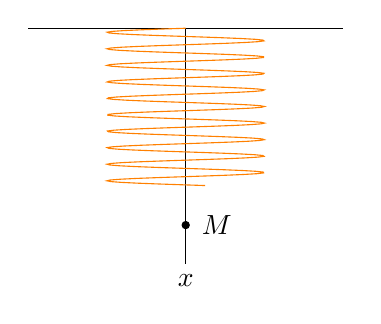
\begin{tikzpicture}
 	\draw  (-2,0) -- (2,0) node[below] {};
 	\draw  (0,0) -- (0,-3) node[below] {$x$};	
 	\draw [orange, domain=0:-2, samples=200] plot({sin(\x r *30},\x);
 	\draw [fill, black, circle] (0,-2.5) circle(0.3ex) node[right] {$M$};
\end{tikzpicture}  } 
\begin{cutout} {0}{8cm}{0pt}{6}
\begin{proof} 
	根据牛顿第二定律,可建立方程:\\
		$\displaystyle~~~F = -k x$ \\
		$\displaystyle~~~F  = Ma =M\frac{d^2 x}{d t} $\\
		$\displaystyle~~~\frac{d^2 x}{d t} = -\frac{k}{M} x$\\
		$\displaystyle~~~\frac{d^2 x}{d t} +\omega ^2 x = 0$\\				
\end{proof}
 \end{cutout} 
由初始位移和初始速度,得初始条件:
	\begin{equation*}
	x(t=0)=x_0, ~~~~ \frac{dx}{dt} \left |_{t=0}  =0 \right.      
	\end{equation*}
  求解辅助方程: $m^2+\omega ^2=0$ \\
  	\begin{equation*}
  	m_{1, 2} =\pm i\omega     
    \end{equation*}
  方程的基本解: 
	\begin{equation*}
		x_{1} =\cos \omega t  , ~~~~	x_{2} =\sin \omega t     
	\end{equation*}
  方程通解: $x(t)=C_1 \cos \omega t +C_2 \sin \omega t $ \\
  初始条件定系数,得特解:$x(t)=x_0 \cos \omega t $ \\
\end{example}

\begin{remark}
这是个常系数二阶齐次线性微分方程,通过辅助方程求解。 
\end{remark}

\begin{example} %7
救解如下小阻尼振动微分方程:
\begin{equation*}
\frac{d^2 u}{d t^2} +2\varepsilon \frac{d u}{dt} +\omega ^2 u = 0 ,  ~~~ (\varepsilon < \omega)   
\end{equation*}
	\begin{proof} 
令 $\displaystyle  u(t)= exp(-\varepsilon t) v(t) $		求微分,得:\\	
\begin{align*}
	\frac{d u}{d t } & =exp(-\varepsilon t) [-\varepsilon v +\frac{d v}{dt}]
	\frac{d^2 u}{d t^2 } & =exp(-\varepsilon t) [\varepsilon ^2 v -2\varepsilon \frac{d v}{dt}+ \frac{d^2 v}{dt^2} ]
\end{align*}
代回原方程并整理得
\begin{equation*}
	\frac{d^2 v}{d t^2} +(\omega ^2 - \varepsilon ^2) u = 0,  ~~~ (\varepsilon < \omega)   
\end{equation*}
令 $k^2 =\omega ^2 - \varepsilon ^2 $, 得简谐振动的微分方程的标准型。由公式 得\\
 $v(t)=C_1 \cos k t +C_2 \sin k t $ \\
方程的通解: $ u(t)= exp(-\varepsilon t) v(t) =exp(-\varepsilon t) [ C_1 \cos k t +C_2 \sin k t] $ \\
	\end{proof}
很明显,振幅呈指数衰减.
\end{example}
%\begin{tikzpicture} 
%	% draw the axis
%	\draw[eaxis] (0,0) -- (5,0) node[below] {$t$};
%	\draw[eaxis] (0,-1) -- (0,1) node[left] {$u$};
%	\draw[elegant,orange,domain=0:5] plot(\x, {sin(\x r *10)*exp(-0.05*\x *10) } );
%\end{tikzpicture} 

\begin{tikzpicture}
	\datavisualization [ scientific axes,  visualize as smooth line/.list={1,2,3,4,5,6,7,8}, 
	style sheet=vary thickness , style sheet=strong colors, all axes={ticks=few}, x axis={label=$t$}, y axis={label=$u$} , style sheet=strong colors ] 
	data [format=function] {
		var set : {2};
		var x : interval [0:10] samples 200;
		func y = sin(\value x r * 10) *exp(-0.05* \value x * 10);
	}
	data [ set=lin, format=function] {
	var set : {1};
	var x : interval [0:10] samples 200;
	func y = 0;
    } ;
\end{tikzpicture}

\begin{example} %8
	求解如下无阻尼强迫振动微分方程:
	\begin{equation*}
		\frac{d^2 u}{d t^2} + \omega ^2 u = p  \sin \omega_0 t 
	\end{equation*}
	\begin{proof} 
		这是个非齐次方程,对应齐次方程的通解已知:\\
        $u(t)=C_1 \cos \omega t +C_2 \sin \omega t $ \\
        只要求出一个特解就行,设非齐次方程的特解为:\\
           $ u(t) =C_0 \sin \omega_0 t $ \\
         代入原方程求待定系数
		\begin{align*}
		C_0(\omega^2-\omega_{0} ^2 ) \sin(\omega_0 t)& =p\sin(\omega_0 t)\\
		C_0 & = \frac{p}{\omega^2-\omega_{0} ^2 }
		\end{align*}
		方程的解为: $ u(t)= C_1 \cos \omega t +C_2 \sin \omega t+ \frac{p}{\omega^2-\omega_{0} ^2 } \sin (\omega_0 t) $ \\
	\end{proof}
\end{example}

\begin{remark}
	如果策动频率与固有频率接近,则出现共振动(振幅很大)
\end{remark}

\begin{tikzpicture} 
	\centering
	% draw the axis
	\draw[eaxis] (0,0) -- (5,0) node[below] {$t$};
	\draw[eaxis] (0,-1) -- (0,1) node[left] {$u$};
	\draw[elegant,orange,domain=0:5] plot(\x, { (1-0.85^2)^(-1) * (sin( \x r *30 ) + sin (0.85*\x r *30 )      )  *0.3       } );
\end{tikzpicture} 

\begin{note}
无阻尼强迫振动微分方程一般式为:
	\begin{equation*}
	\frac{d^2 u}{d t^2} + \omega ^2 u = f(t)
\end{equation*}
当策动函数为多项式函数,三角函数时, 可用待定系数法确定特解。对于其他的情况,一般常采用常数变易法求解。
\end{note}

%%%%%%%%%%%%%%%%%%%%%%%%%%%%%%
\subsection{常微分方程求解方法}
\subsubsection{一阶常微分方程}
\begin{example} %9
	求解如下一阶常系数线性非齐次常微分方程:
	\begin{equation*}
	 y'+py=f(x)
	\end{equation*}
	\begin{proof} 
		对应的齐次方程是衰减数学模型,有解:\\
		$w=C_0 exp(-px)$ \\
		应用常数变易法,设非齐次方程的解为:\\
		$ y(x) =u(x) exp(-px)$ \\
		代入原方程得
		\begin{align*}
		exp(−px)u′ &= f(x)\\
		u(x) &= \int exp(px) f (x)dx + C
		\end{align*}
		原方程的解为: $ y(x)=C exp(-px)+exp(-px) \int exp(px)f(x)dx $ \\
	\end{proof}
\end{example}

\subsubsection{二阶常微分方程}
\begin{example} %10
	求解如下二阶常系数线性非齐次常微分方程:
	\begin{equation*}
		y''+py'+qy=f(x)
	\end{equation*}
	\begin{proof} 
	对应的齐次方程为:
	\begin{equation*}
	y''+py'+qy=0
   \end{equation*}
	其特征方程为:
 \begin{equation*}
	\lambda^2 +p\lambda +q=0
  \end{equation*}
  解有三种情况:
  \begin{table} [H]
\begin{tabular}{ccc}
	两相异实根:& $\lambda_1 \ne \lambda_2 $ & \\
	两相同实根:& $\lambda_1 = \lambda_2 $  &\\
	两共轭复根:& $\lambda_1=\alpha+i\beta $, & $\lambda_2=\alpha-i\beta$\\ 
\end{tabular}
 \end{table}
对应的齐次方程的通解也有三种情况:
  \begin{table} [H]
	\begin{tabular}{cccc}
		异实根:y=& $C_1 exp(\lambda_1 x)+ C_2 exp (\lambda_2 x) $ & \\
		同实根:y=&$(C_1+C_2x)  exp (\lambda_1 x) $  &\\
		共轭复根:y=& $ exp(\alpha x)  [C_1 \cos (\beta x)+ C_2 sin (\beta x)] $\\ 
	\end{tabular}
\end{table}
根据自由项的特点,再通过待定系数法 或常数变易法求解非齐次常微分方程。
	\end{proof}
\end{example}

\begin{example} %10
	求如下二阶常齐次常微分方程的通解:
	\begin{equation*}
		u''-k^2u'=0
	\end{equation*}
	\begin{proof} 
		特征方程为:
		\begin{equation*}
			\lambda^2 -k^2=0
		\end{equation*}
		 存在两相异实根: $\lambda_1=k, ~~~ \lambda_2 =-k $ \\
		通解为:~~~~~~u(t)= $C_1 exp(k x)+ C_2 exp (-k x) $  \\
		写成双曲函数形式为: u(t)= $D_1 cosh(k x)+ C_2 sinh (k x) $  \\
	\end{proof}
\end{example}

\begin{example} %11
	求如下二阶常齐次常微分方程的初值问题:
$\begin{cases}
	u'' =f, (x>0)\\
	u(0)=0, u'(0)=0
\end{cases}$
	\begin{proof} 
		对方程两边求积分
		\begin{equation*}
		u'=\int_{0}^{\xi} f(s) ds +c_1
		\end{equation*}
		\begin{equation*}
		u(x)=\int_{0}^{x}   d\xi  \int_{0}^{\xi} f(s) ds +c_1x  +c_2
	    \end{equation*}
       代入零值条件,得  $c_1=0, c_2=0$, 现交换积分次序\\
 		\begin{equation*}
     	u(x)=\int_{0}^{x}   ds  \int_{s}^{x} f(s) d\xi = \int_{0}^{x}  (x-s)f(s) ds 
         \end{equation*}      
	\end{proof}
\end{example}
\begin{note}
	注意(1)定积分与变上限积分之间的关系 (2)交换积分次序时,定积分上下限的变化。
\end{note}

\begin{example} %12
	求如下二阶常齐次常微分方程的初值问题:\\
	$\begin{cases}
		u'' =f, (x>0)\\
		u(0)=\alpha, u'(0)=\beta
	\end{cases}$
	\begin{proof} 
		显然,v(x)	=$\alpha$+$\beta$x 与 u(x) 享有相同的初值条件。所以它是如下齐次方程的解:\\
		$\begin{cases}
			u'' =0, (x>0)\\
			u(0)=\alpha, u'(0)=\beta
		\end{cases}$\\
	令 u(x)=v(x)+w(x),。 则 w(x) 满足如下零值问题,\\	
	$\begin{cases}
	w'' =0, (x>0)\\
	w(0)=\alpha, w'(0)=\beta
     \end{cases}$\\	  
    由上题的解,写出原方程的解:\\
		\begin{equation*}
			u(x)=\alpha+\beta x +  \int_{0}^{x}  (x-s)f(s) ds 
		\end{equation*}      
	\end{proof}
\end{example}

\begin{note}
	注意本题是如何把非零初值问题转化为零初值问题的
\end{note}

\begin{example} %13
	用常数变易法求解常微分方程初值问题:\\
	$\begin{cases}
		u'' +\omega ^2 u =f, (t>0)\\
		u(0)=0, u'(0)=0
	\end{cases}$
	\begin{proof} 
	齐次方程的通解为:
	\begin{equation*}
		u=C_1 \cos(\omega t)+C_2 \sin(\omega t)
	\end{equation*}     
    作常数变易,即设非齐次方程的解可写为 
	\begin{equation*}
	u=C_1(t) \cos(\omega t)+C_2(t) \sin(\omega t)
   \end{equation*}    
   求导,有
		\begin{equation*}
			u‘=[C'_1(t) \cos(\omega t)+C'_2(t) \sin(\omega t)] + [  - \omega C_1(t) \sin(\omega t)+ \omega C_2(t) \cos(\omega t)  ]
		\end{equation*}    
	令   [$C'_1(t) \cos(\omega t)+C'_2(t) \sin(\omega t)$] =0,  ~~~ $\dots$ (1) 有
	\begin{equation*}
		u'= [  - \omega C_1(t) \sin(\omega t)+ \omega C_2(t) \cos(\omega t)  ]
	\end{equation*}    
	进行二次求导:
	\begin{equation*}
		u‘‘= [  - \omega C'_1(t) \sin(\omega t)+ \omega C'_2(t) \cos(\omega t)  ] -\omega^2 u
	\end{equation*}  
   把上次代回原方程,得:
   	\begin{equation*}
   	[  - \omega C'_1(t) \sin(\omega t)+ \omega C'_2(t) \cos(\omega t)  ] =f       ~~~~  \left( 2\right)
   \end{equation*}  
联立(1)(2), 得方程组:\\  	\vspace{0.3cm}
$\begin{bmatrix}
	 \cos(\omega t) & \sin(\omega t) \\ 
	 -\omega \sin(\omega t) & \omega\cos(\omega t)
\end{bmatrix} $
$\begin{bmatrix}
	C'_1(t)\\ 
	C'_2(t)
\end{bmatrix} $ =
$\begin{bmatrix}
	0\\ 
	f
\end{bmatrix} $ \\
解得:\\  	\vspace{0.3cm}
$\displaystyle \begin{cases}
	C'_1(t)=\frac{1}{\omega} \sin(\omega t) f \\ 
	C'_2(t)=\frac{1}{\omega} \cos(\omega t) f 
\end{cases} $ \\
积分得:\\  	\vspace{0.3cm}
$\displaystyle \begin{cases}
	C_1(t)=\frac{1}{\omega} [\int_{0}^{\tau} \sin(\omega \tau) f(\tau)  d\tau +c_1 ]\\ 
	C_2(t)=\frac{1}{\omega} [\int_{0}^{\tau} \cos(\omega \tau) f(\tau)  d\tau +c_2 ]\
\end{cases} $ \\
原方程的解为:\\
\begin{equation*}
	u=\frac{1}{\omega}\cos(\omega t)[\int_{0}^{\tau} \sin(\omega \tau) f(\tau)  d\tau +c_1 ] +\frac{1}{\omega} \sin(\omega t) [\int_{0}^{\tau} \cos(\omega \tau) f(\tau)  d\tau +c_2 ]
\end{equation*}   
代入初值条件, 得 $c_1=c_2=0$, 最终得:  
原方程的解为:\\
\begin{equation*}
	u=\frac{1}{\omega}\int_{0}^{\tau} \sin\omega (t-\tau)  f(\tau)  d\tau
\end{equation*}   
\end{proof}
\end{example}

\begin{note}
	 常数变易后的主要目标变为求$C_1(t), C_2(t) $.
\end{note}

\subsubsection{变系数二阶常微分方程}
\begin{example} %14
	求解欧拉方程:
\begin{equation*}
	x^2 \frac{d^2 y}{d x^2} +x \frac{d y}{d x} +n^2 y =0 
\end{equation*}     

	\begin{proof} 
		令 $x=exp(t) $ (t=ln x),代入原方程可转化为:
		\begin{equation*}
		 \frac{d^2 y}{d t^2}  +n^2 y =0 
		\end{equation*}     
		这是振动方程,有通解:
		\begin{equation*}
			y(t)=C_1 \cos n t +C_2 \sin n t
		\end{equation*}    
		原方程的解为:\\
    	\begin{equation*}
    	y(t)=C_1 \cos n \ln x +C_2 \sin n \ln x
        \end{equation*}    
	\end{proof}
\end{example}

\begin{example} %15
	求解如下形式的欧拉方程:
	\begin{equation*}
		x^2 \frac{d^2 y}{d x^2} +2x \frac{d y}{d x} -n(n+1) y =0 
	\end{equation*}     
	
	\begin{proof} 
		令 $x=exp(t) $ (t=ln x), 代入原方程可转化为:
		\begin{equation*}
			\frac{d^2 y}{d t^2} + \frac{dy}{dt}-n(n+1) y =0 
		\end{equation*}     
		其特征方程为
		\begin{equation*}
		\lambda^2 +\lambda -n(n+1) =0	
		\end{equation*}    
	    其解两相异实根: $\lambda_1=n, \lambda_2= -(n+1)$,
		原方程的能解:
		\begin{equation*}
		y(t)=C_1 \exp (nt) +C_2 \exp (-(n+1) t)
		\end{equation*}    
	   即:
	  	\begin{equation*}
	  	y(t)=C_1 x^n +C_2 x^{-(n+1) }
	   \end{equation*}     
	\end{proof}
\end{example}

\begin{note}
	由特征方程写通解是门艺术
\end{note}

\begin{example} %16
	幂级数方法求解 n 阶厄米方程
	\begin{equation*}
		\frac{d^2 y}{d x^2} -2x \frac{d y}{d x} +2n y =0 
	\end{equation*}     
	
	\begin{proof} 
	设方程有级数解
		\begin{equation*}
		y=\sum_{k=0}^{\infty} c_k x^k
		\end{equation*}     
	 求导得:\\
	$\begin{cases}
	 y' = \sum_{k=1}^{\infty} k c_k x^{k-1} \\
	 y'' = \sum_{k=2}^{\infty} k (k-1) c_k x^{k-2} =  \sum_{k=0}^{\infty} (k+2) (k+1) c_{k+2} x^k
	 \end{cases}$ \\
    代回原方程,得:
   	\begin{equation*}
    \sum_{k=0}^{\infty} [ 2nc_k -2kc_k +(k+2)(k+1) c_{k+2}  ] x^k  =0
    \end{equation*}   
    各项系数为零,即: 
     \begin{equation*}
    2nc_k -2kc_k +(k+2)(k+1) c_{k+2} =0
    \end{equation*}   
    得系数递推式:
    \begin{equation*}
    c_{k+2} = \frac{ 2(k-n)}{(k+2)(k+1) } c_k, ~~  \left( k=0,1,2,3, ...  \right)
    \end{equation*}   
   分偶数阶和奇数阶来写,偶数阶有: \\
   	$\displaystyle \begin{cases}
    c_2 =- \frac{2n}{2!} c_0\\
    c_4 = \frac{2^2n(n-2)}{4!} c_0 \\
    c_6 = -\frac{2^3n(n-2)(n-4)}{6!} c_0 \\
    c_{2m} = (-1) ^m \frac{2^mn(n-2)(n-4) ... (n-2m+2)  } {(2m)!} c_0
   \end{cases}$ \\
   同理,奇数阶有:\\
   { $\displaystyle
    c_{2m+1} = (-1) ^m \frac{2^m (n-1) (n-3)(n-5)...(n-2m+1)  } {(2m+1)!} c_1$}\\
  所有系数求解,即幂级数求得,\\
    $\displaystyle \begin{cases}
 	y_1(x)  = [1- \frac{2n}{2!} x^2+ \frac{2^2n(n-2)}{4!} x^4 -...  ] \\
 	y_2(x)  = [x- \frac{2(n-1)}{3!} x^3+ \frac{2^2(n-1)(n-3) }{5!}x^5 -...  ]
   \end{cases}$ \\
    原方程的解为:
     \begin{equation*}
    y(x) =c_0y_1(x)+c_1 y_2(x).
    \end{equation*}   
	\end{proof}
\end{example}

\begin{note}
	级数法更是一门艺术
\end{note}

\subsection{傳里叶级数和傅里叶变换}
\subsubsection{傳里叶级数 }
\textbf{\large 三角式}:\\
{\large  $\displaystyle f(x) =\frac{a_0}{2} \sum_{n=1}^{\infty}  \left(  a_n \cos~ \frac{n\pi}{l} x +  b_n \cos~ \frac{n\pi}{l} x  \right) $ }\\	
{\large $\displaystyle a_n =\frac{1}{l}  \int_{-l}^{l}  f(\xi )   \cos~ \frac{n\pi}{l} \xi d\xi  $ }\\	
{\large $\displaystyle b_n =\frac{1}{l}  \int_{-l}^{l}  f(\xi )   \sin~ \frac{n\pi}{l} \xi d\xi   $ }\\	

\textbf{ \large 复数式:} \\  \vspace{0.3cm}
{\large  $\displaystyle f(x) =\sum_{n=-\infty}^{+\infty}  c_n e^{i\omega_n x} $ }\\	
{\large $\displaystyle c_n =\frac{1}{2l}  \int_{-l}^{l}  f(\xi)    e^{-i\omega_n x}  d\xi  $ }\\	
其中:{\large $\displaystyle   \omega_n=\frac{n\pi}{l} ,  n=...,-3,-2,-1,0,1,2,3,...   $} \\

\textbf{{\large 周期($2l$) 与 非周期 ($l~\to ~\infty$)}} \\
{\large  $\displaystyle f(x) =\lim_{l\to \infty} \sum_{n=-\infty}^{+\infty}  c_n e^{i\omega_n x} $ }\\	
\hspace{5em}{\large $\displaystyle =\lim_{l\to \infty} \sum_{n=-\infty}^{+\infty}  \frac{1}{2l}  [\int_{-l}^{l}  f(\xi)  e^{-i\omega_n x}  d\xi ]  e^{i\omega_n x}  $ }\\	
\hspace{5em}{\large $\displaystyle =\frac{1}{2\pi} \int_{-\infty}^{+\infty}  [\int_{-l}^{l}  f(\xi)  e^{-i\omega x}  d\xi ]  e^{i\omega x} d\omega $ }\\
\hspace{5em}{\large $\displaystyle =\frac{1}{2\pi} \int_{-\infty}^{+\infty}  G(\omega) e^{i\omega x} d\omega $ }\\

\begin{note}
$	1, \cos(x), \sin (x), \cos(2x), \sin (2x), ..., \cos(nx), \sin (nx) $, 构成正交完全集,
$\left\{  exp(i\omega x)  \right\}$  也构成正交完全集。\\
\end{note}
\begin{tikzpicture}
	 \draw[eaxis] (0,0) -- (8,0) node[below] {$x$};
	\draw[eaxis] (0,0) -- (0,4) node[right] {$y$};
    \draw [blue, thick, x=0.0185cm, y=2cm,
	declare function={
		sines(\t,\a,\b,\c,\d,\e )=1 + \a*sin(\t)+\b*sin(\t*\d)+\c*sin(\t*\e));
	}]
	plot [domain=0:360, samples=144, smooth] (\x,{sines(\x,0.5, 0.2, 0.1, 3, 5)}); 
\end{tikzpicture}
\begin{equation*}
y=1 + 0.5\sin(x)+0.6\sin(3x)+0.7\sin(5x)
\end{equation*}    

\begin{example} %16
求函数的傳里叶展开式:
    $\displaystyle f(x)=\begin{cases}
		1 , ~~~ x \in [0, \pi] \\
		-1 ,~~~ x \in [-\pi, 0] \
    \end{cases}$ \\
	\begin{proof} 
		这是个奇函数, 展开式中只有sin函数, 只需计算 $b_n$\\
		\begin{equation*}
	    b_n =\frac{1}{\pi}  \int_{-\pi}^{\pi}  f(x) \sin~ \frac{n\pi}{\pi} x dx  
        \end{equation*}     
        代入 f (x), 得:\\
		\begin{align*}
         b_n &=\frac{1}{\pi}  [ \int_{-\pi}^{0}  \sin n x dx - \int_{0}^{\pi}  \sin~nx dx] \\
                 &=\frac{2}{\pi}  \int_{0}^{\pi}  \sin nx dx  \\
                 &=\frac{2}{n\pi} [\cos nx] \left\|_0 ^\pi  \right. \\
                 &=\frac{2}{n\pi} [ (-1) ^n -1]
        \end{align*}
        	\begin{equation*}
        	f(x) = \frac{4}{\pi} \sum_{n=0}^{\infty}  \frac{1}{2k+1} \sin(2k+1) dx  
        \end{equation*}       
    	\end{proof}
\end{example}

\subsubsection{傳里叶变换 }
由非周期的傳里叶级数,获得傳里叶变换公式:\\
$\displaystyle \begin{cases}
	G(\omega) =\int_{-\infty}^{+\infty}  f(x) e^{-i\omega x} dx \\
	f(x) =\frac{1}{2\pi} \int_{-\infty}^{+\infty}  G(\omega) e^{i\omega x} d\omega
\end{cases}$ \\

{可转化为对称形式}\\ 
$\displaystyle \begin{cases}
	G(\omega) =\frac{1}{\sqrt{2\pi}} \int_{-\infty}^{+\infty}  f(x) e^{-i\omega x} dx  \equiv F[f(x)]\\
	f(x) =\frac{1}{\sqrt{2\pi}}  \int_{-\infty}^{+\infty}  G(\omega) e^{i\omega x} d\omega  \equiv F^{-1}[G(\omega)]
\end{cases}$ \\

\begin{example} %16
	在量子力学中,一维体系中的一个状态在坐标表象中的波函数为:
	\begin{equation*}
	\Psi(x)=\frac{1}{\sqrt{2\pi \hbar}}  \int_{-\infty}^{+\infty} c(p) e^{\frac{i}{\hbar} px} dp 
    \end{equation*}   
   求该状态在动量表象中的波函数 c (p).
	\begin{proof} 
		把波函数改写成  \\
		\begin{equation*}
		\Psi(x)= \frac{1}{\sqrt{2\pi }} \int_{-\infty}^{+\infty} \sqrt{\hbar} c(p) e^{i\frac{p}{\hbar} x} d(\frac{p}{\hbar})  
		\end{equation*}     
	 根据对称型傅里叶变换公式,有: \\
	$\displaystyle \begin{cases}
		\sqrt{\hbar} c(p) = \frac{1}{\sqrt{2\pi }} \int_{-\infty}^{+\infty} \Psi(x) e^{-i\frac{p}{\hbar} x} dx\\
		c(p) = \frac{1}{\sqrt{2\pi \hbar }} \int_{-\infty}^{+\infty} \Psi(x) e^{-\frac{i}{\hbar} px} dx
	\end{cases}$ \\  
	\end{proof}
\end{example}

\subsection{作业}
~~ \hspace*{\fill} \\ 
1、求函数的傳里叶展开式:
$\displaystyle f(x)=\begin{cases}
	\pi +x , ~~~ x \in [-\pi, 0] \\
	\pi -x ,~~~ x \in   [0, \pi] 
\end{cases}$ \\
2、分离变量法求方程\\
\begin{equation*}
	\frac{dy}{dt}	=  r y (1-\frac{y}{K}), ~~~~ y(t_0) = y_0
\end{equation*}
3、	幂级数方法求解方程\\
\begin{equation*}
	\frac{d^2 y}{d x^2} -2x \frac{d y}{d x} +2n y =0 
\end{equation*}     